%duvida 1: qual melhor pessoa para usar em frazes
%   nessa etapa precisamos (ingles)
%   nessa etapa é preciso
%   nessa etapa precisei
%   nessa etapa foi necessário       usar essa



\chapter{Implementação}

%Essa seção não é muito relevante para o resultado final, não sei se escrevo ela
\section{Configuração do Ambiente}

%Mover para fundamentação teórica
\subsection{Usando os Buffers do OpenGL e GLSL}

\subsubsection{Descrição dos vértices}

\subsubsection{Implementação do sistema de Navegação}


\section{Criando Malha de Triângulos}
A maneira que um jogo renderiza seu terreno no final das contas é sobre uma
malha, uma malha é um conjunto de vértices que podem representar fragmentos
de uma superfície do terreno.

Para representar um segmento de plano precisamos de pelo menos $3$ vértices, 
já que com dois podemos apenas representar segmentos de retas. Um plano precisar
ter um mesmo vetor normal para todo o plano.

A malha segue pelo plano $XZ$, e cada vértice do plano vai ter uma altura
$y$ definida mais tarde por ruído. Se quisermos que o conjunto de pontos pertença
ao memos segmento de plano precisamos que os quatro pontos respeitem a mesma
equação do plano.

Se usarmos como plano $4$ pontos em $R3$
\begin{equation}\label{comp_sign_inter_sem_peso_aux}
    V = \{v_{0}(0, y_{0}, 0), v_{1}(0, y_{1}, 1), v_{2}(1, y_{2}, 0), v_{3}(1, y_{3}, 1)\}
\end{equation}
Para montar a equação do plano temos $\{y_{0}, y_{1}, y_{2}\}$ como valores livres e $y_{3}$
vai depender dos valores de $\{v_{0}, v_{1}, v_{2}\}$

%Aqui vai o cálculo da equação do plano ou do vetor normal para mostrar o que
%acabei de afirmar acima
%Calculando o vetor normal associado ao plano formado por $\{v0, v1, v2\}$
%$v0v1 = (0, y1-y0, 1)$
%$v0v2 = (1, y2-y0, 0)$

mas não é isso que queremos, queremos que todos os pontos tenha valores de $y$
livres, portanto, será uma malha de triângulos. Então pro conjunto de vértices
acima temos dois triângulos associados:
$T_{1} = \{v_{0}, v_{1}, v_{2}\}, T_{2} = \{v_{3}, v_{1}, v_{2}\}$

\begin{algorithm}[H]\label{comp_vertice_site}
  $delta_{y} = v_{y} - p_{y}$ \\
  \uSe{$delta_{y} < 0$}{
    é verdade que $v < p$.
  }  
  \uSenaoSe{$delta^{2}_{y} < v_{d}$}{
    é verdade que $v < p$.
  }
  \uSenaoSe{$delta^{2}_{y} = v_{d}$ e $v_{x} < p_{x}$}{
    é verdade que $v < p$.
  }
  \uSenao{
    não é verdade que $v < p$.
  }  
  \caption{Comparação entre vértice e \textit{site}.}
\end{algorithm}

\begin{algorithm}[H] %or another one check
 \caption{How to write algorithms}
     \SetAlgoLined

     \While{not at end of this document}{
      read current\;
      \eIf{understand}{
       go to next section\;
       current section becomes this one\;
       }{
       go back to the beginning of current section\;
      }
     }

\end{algorithm}


\begin{align}
    A \in Z^{2} \\
    mix(A, B, c) &= (1-c) * A + c*B \\
    mix(A, B, c) &= (1-c) * A + c*B \\
\end{align}






\section{Aplicando Ruído de Perlin nos Vértices}

\subsection{Manipulando ruído para criar Biomas}
\subsubsection{PLAINS}

\begin{figure}[H]
    \centering
    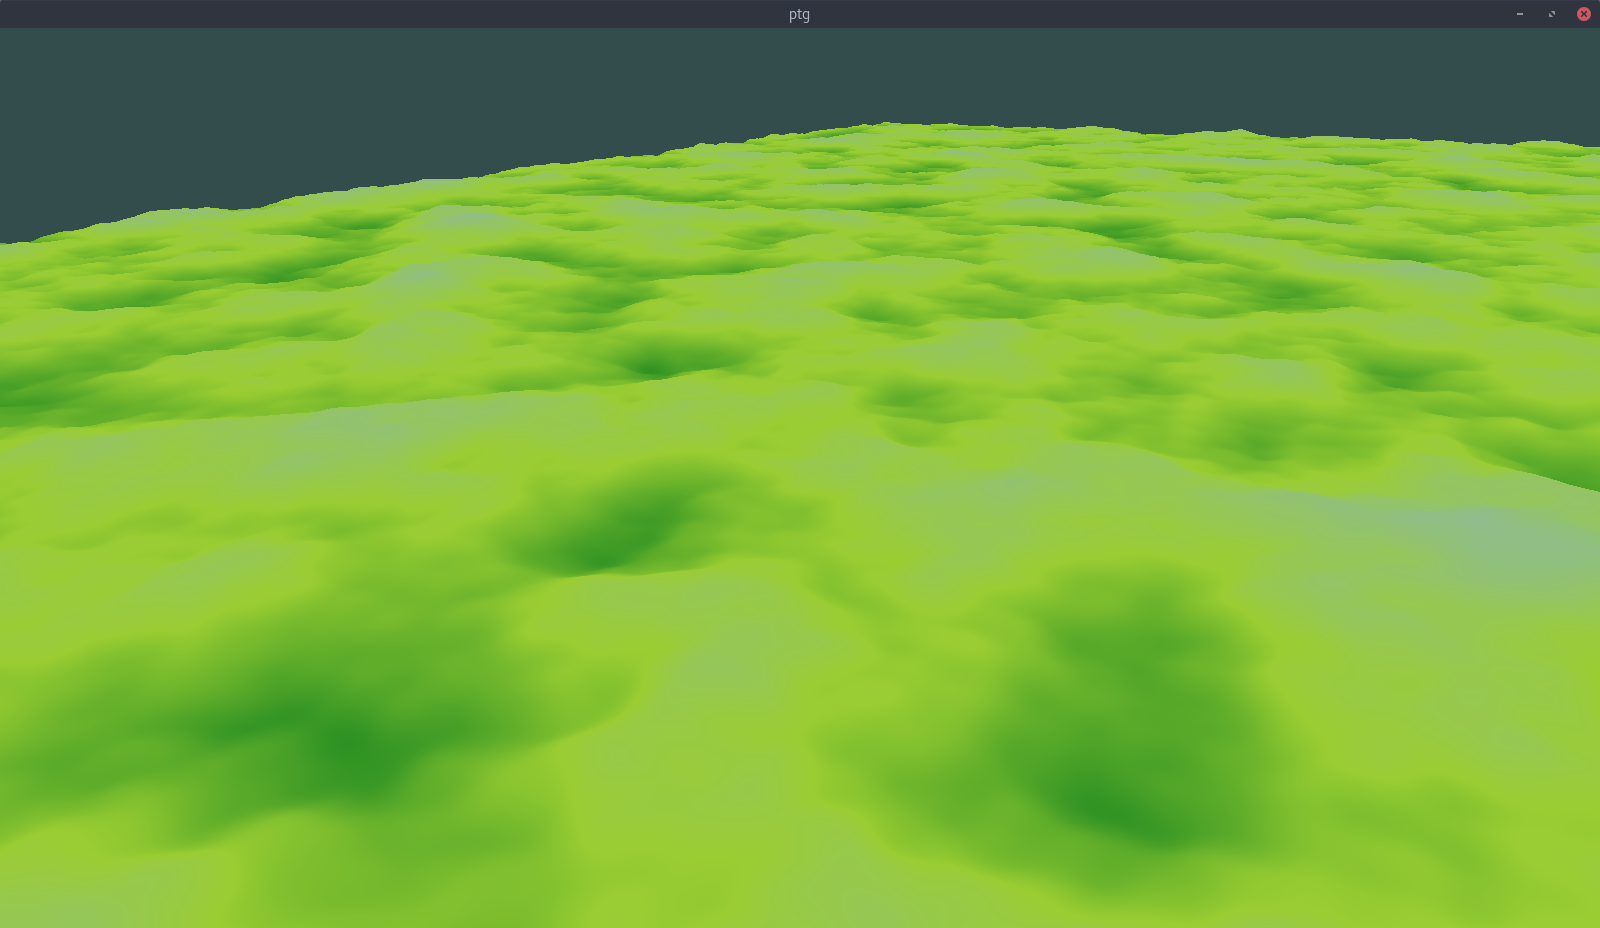
\includegraphics[width=0.5\textwidth]{figuras/bssPlains.png}
    \caption{Consumo}
    \label{fig:bssPlains}
\end{figure}

\subsubsection{MONTAINS}


\begin{figure}[H]
    \centering
    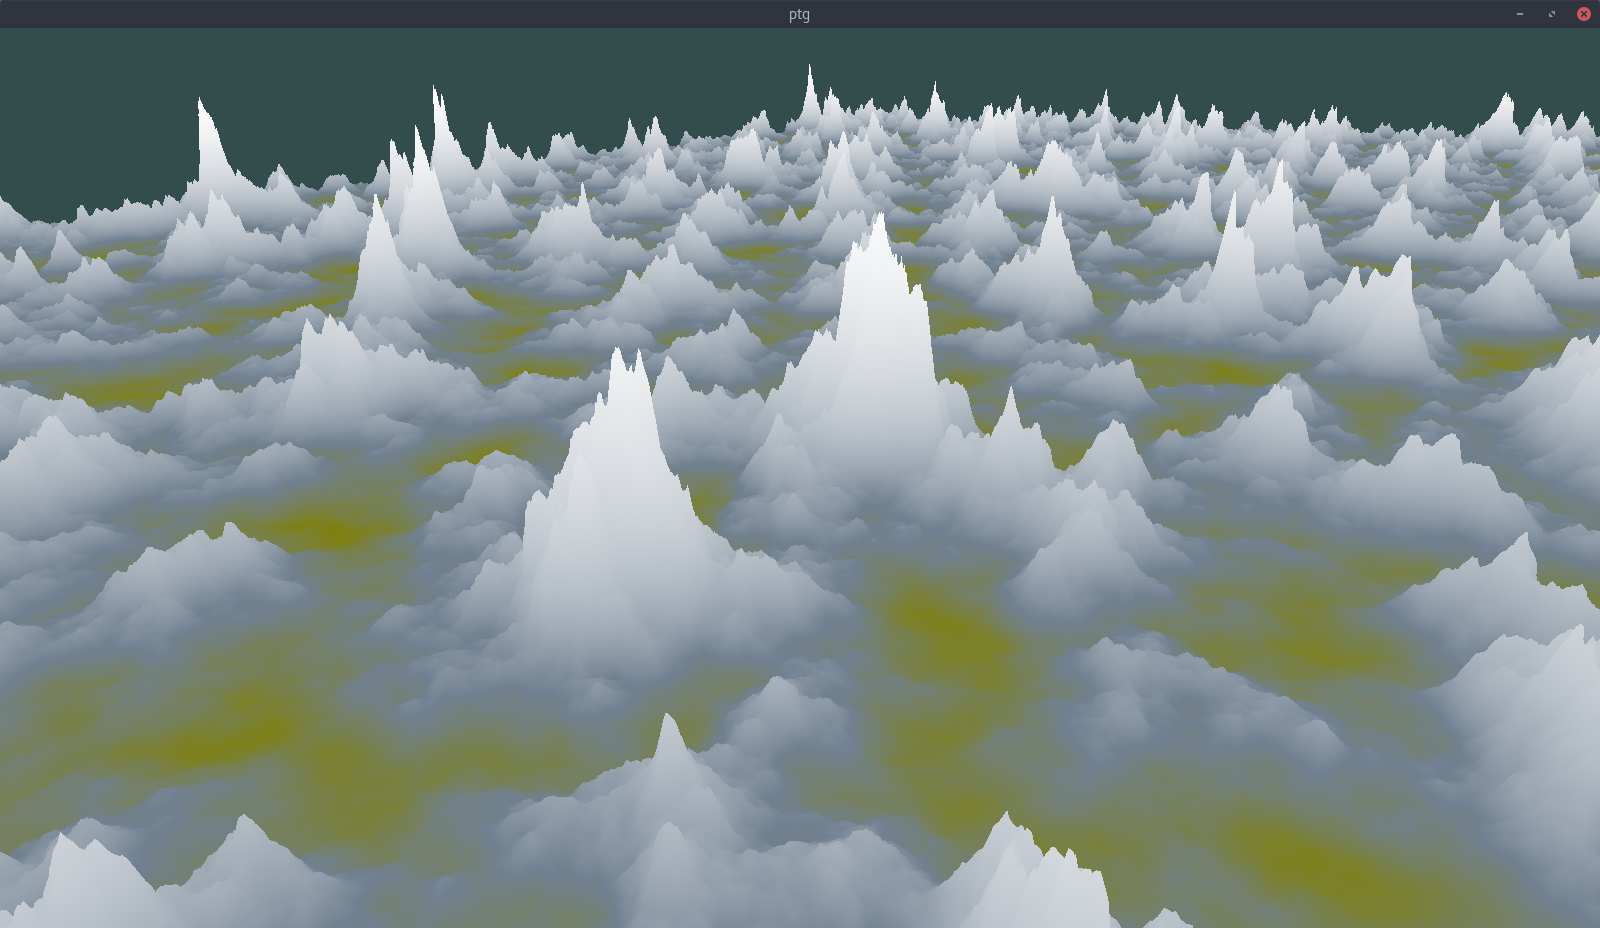
\includegraphics[width=0.5\textwidth]{figuras/bssMontains.png}
    \caption{Consumo}
    \label{fig:bssMontains}
\end{figure}

\subsubsection{VALLEY}


\begin{figure}[H]
    \centering
    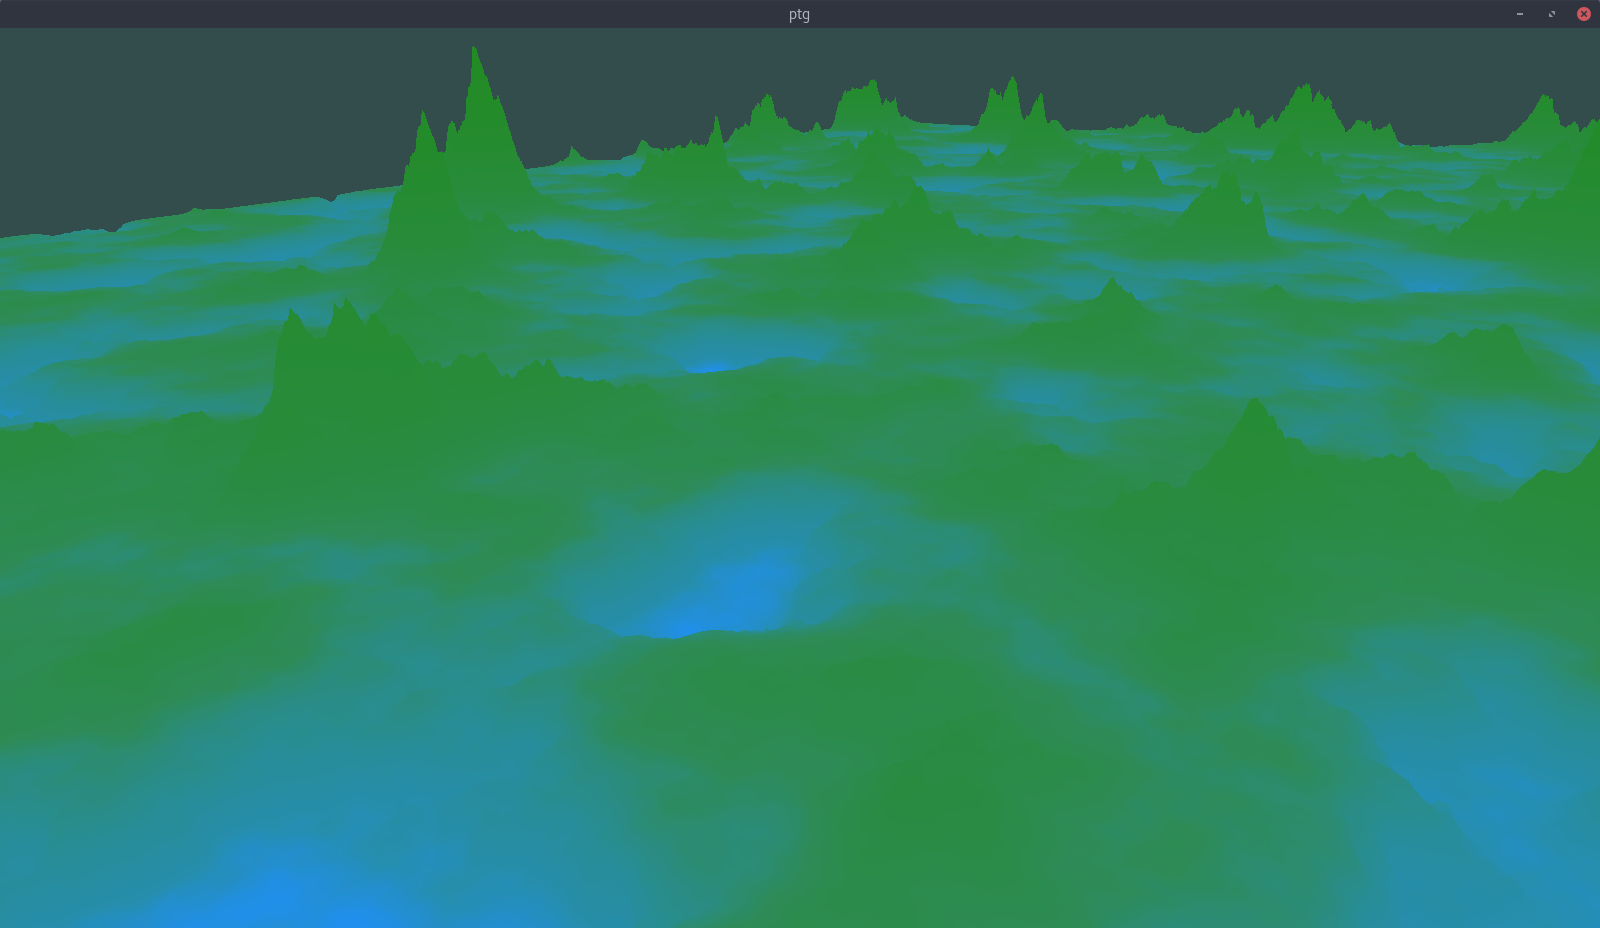
\includegraphics[width=0.5\textwidth]{figuras/bssValley.png}
    \caption{Consumo}
    \label{fig:bssValley}
\end{figure}

\subsubsection{DESERT}


\begin{figure}[H]
    \centering
    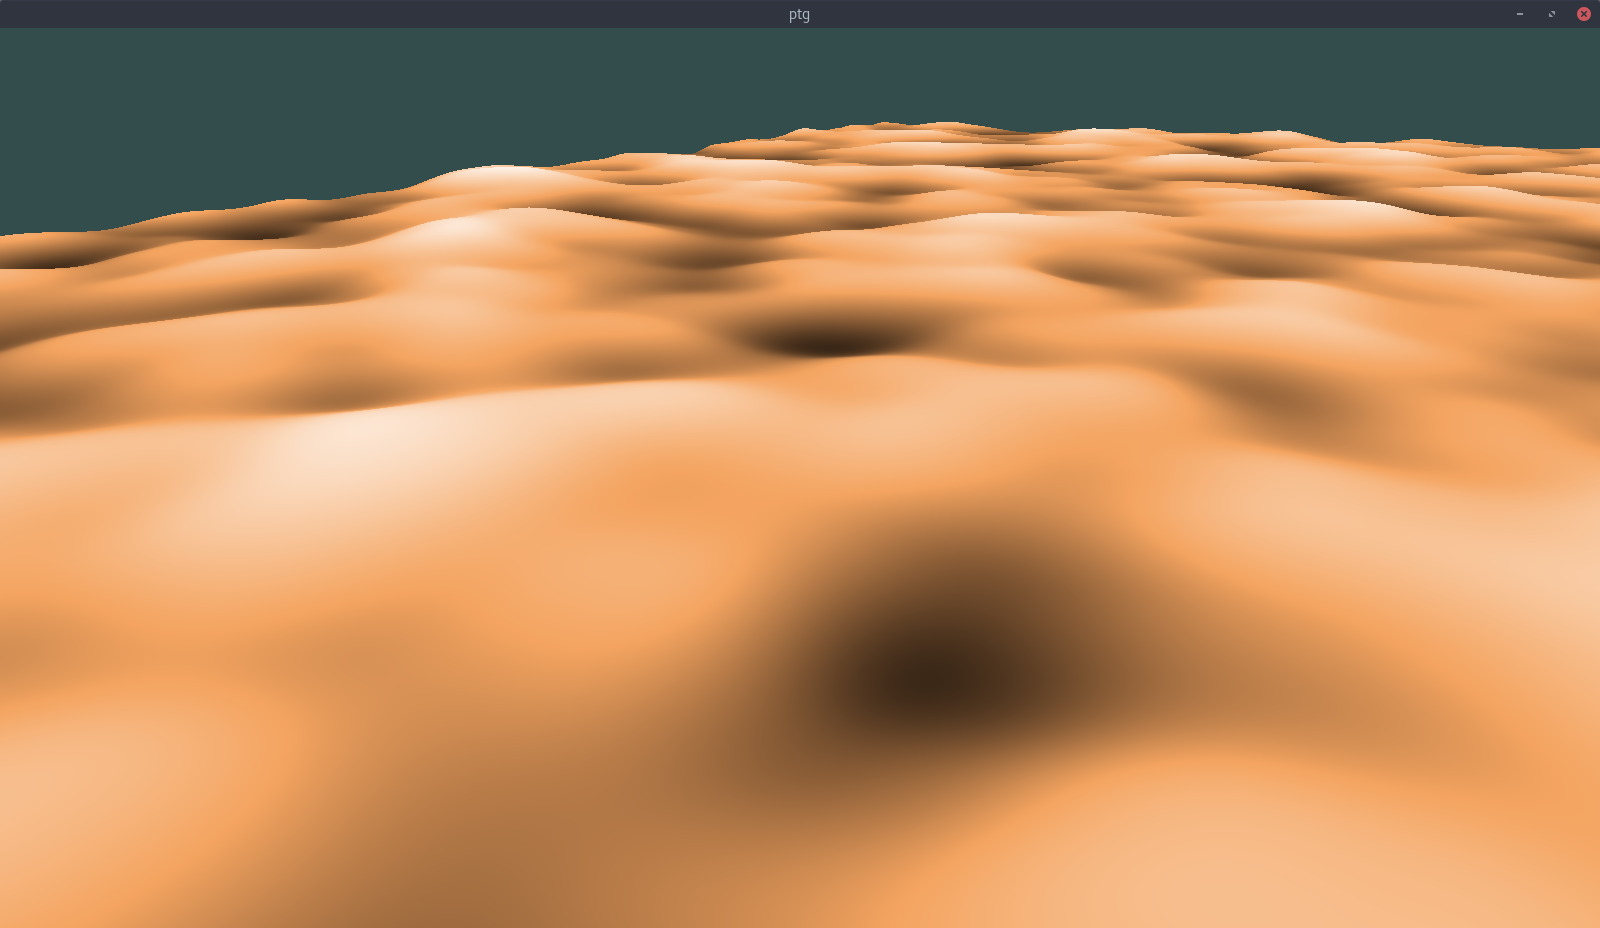
\includegraphics[width=0.5\textwidth]{figuras/bssDesert.png}
    \caption{Consumo}
    \label{fig:bssDesert}
\end{figure}

\subsubsection{CANYONS}


\begin{figure}[H]
    \centering
    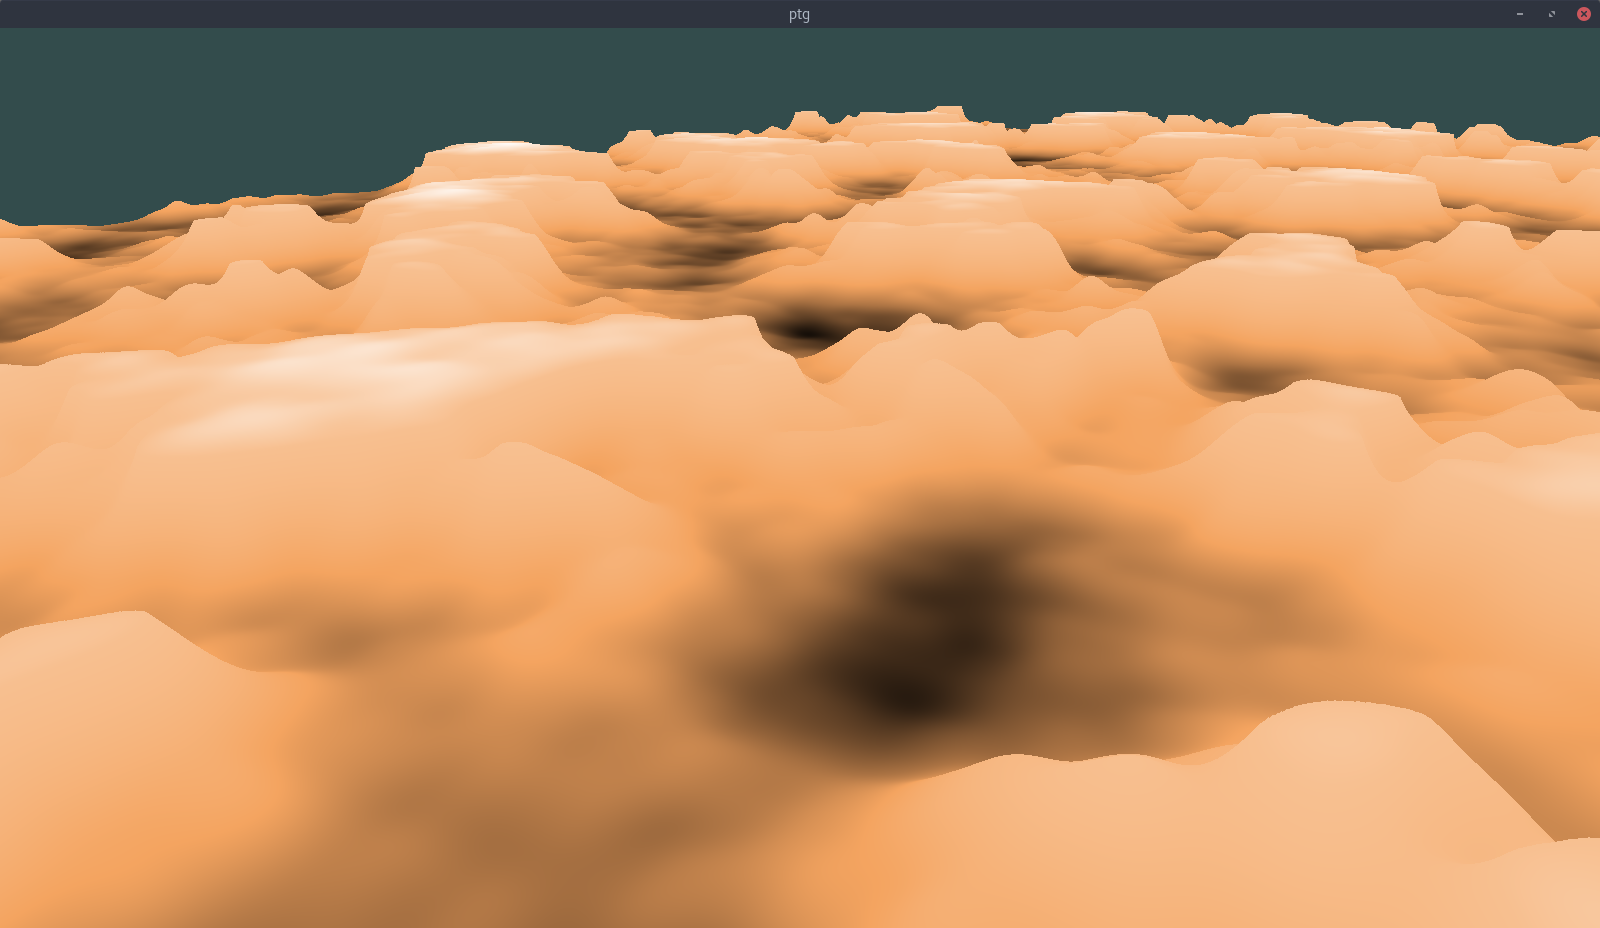
\includegraphics[width=0.5\textwidth]{figuras/bssCanyons.png}
    \caption{Consumo}
    \label{fig:bssCanyons}
\end{figure}

\section{Separando Áreas de Biomas}

\section{Detectando fronteira entre Biomas}